\documentclass{standalone}
\usepackage{tikz}
\usetikzlibrary{patterns, positioning}

\begin{document}
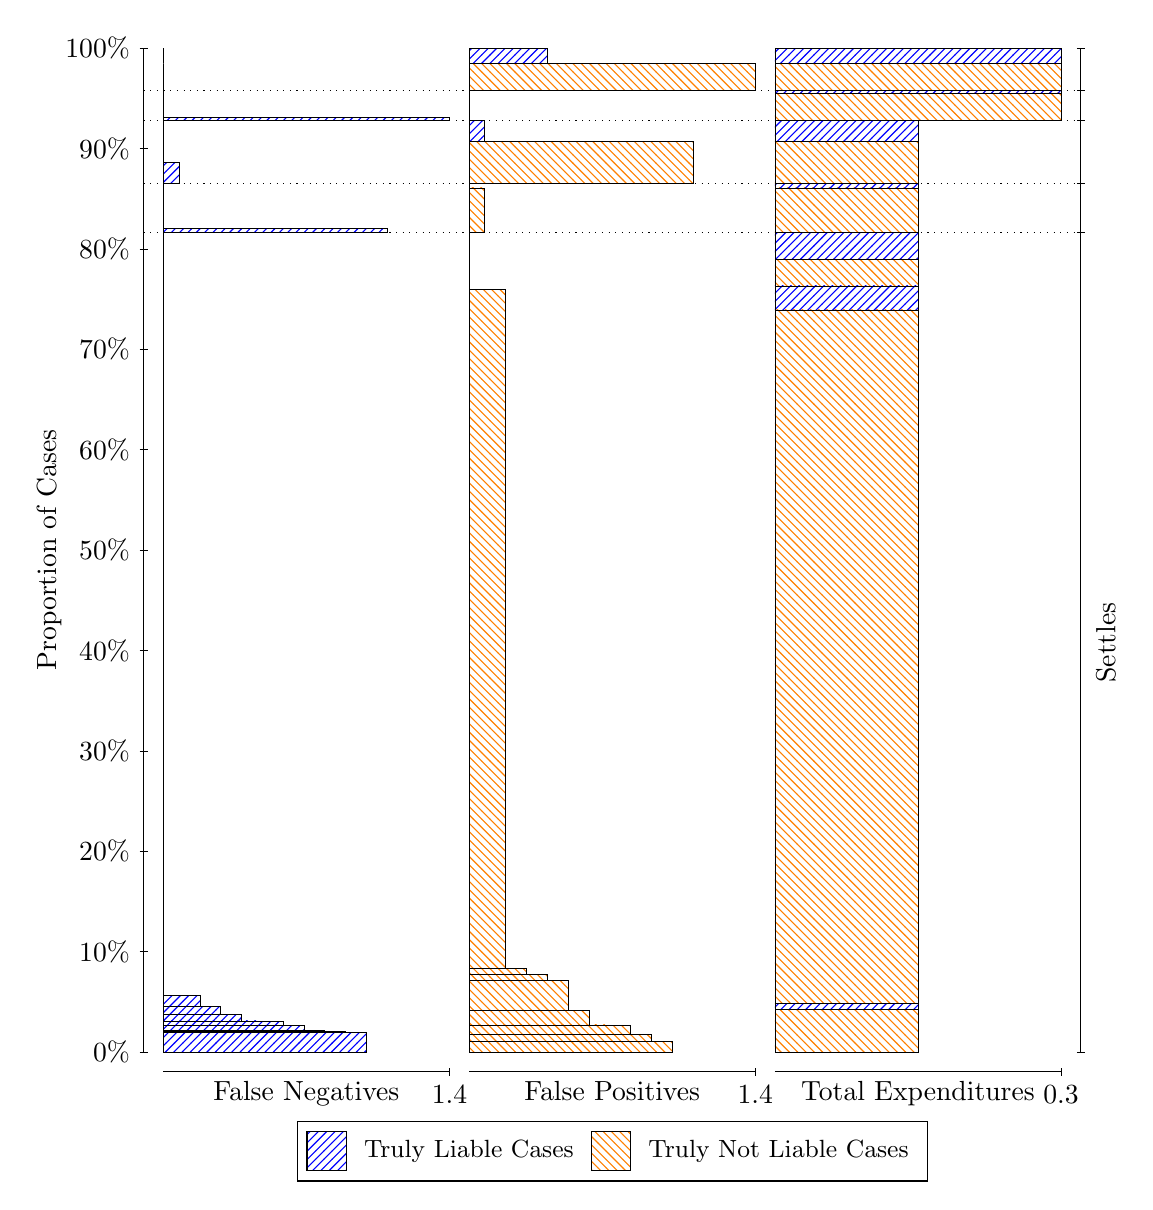
\begin{tikzpicture}
\draw[black, very thin] (1.5,1.75) -- (1.5,14.5);
\node[rotate=90, anchor=center] at (0.3, 8.125) {Proportion of Cases};
\draw[black, very thin] (1.45,1.75) -- (1.55,1.75);
\node[anchor=east] at (1.45, 1.75) {0\%};
\draw[black, very thin] (1.45,3.025) -- (1.55,3.025);
\node[anchor=east] at (1.45, 3.025) {10\%};
\draw[black, very thin] (1.45,4.3) -- (1.55,4.3);
\node[anchor=east] at (1.45, 4.3) {20\%};
\draw[black, very thin] (1.45,5.575) -- (1.55,5.575);
\node[anchor=east] at (1.45, 5.575) {30\%};
\draw[black, very thin] (1.45,6.85) -- (1.55,6.85);
\node[anchor=east] at (1.45, 6.85) {40\%};
\draw[black, very thin] (1.45,8.125) -- (1.55,8.125);
\node[anchor=east] at (1.45, 8.125) {50\%};
\draw[black, very thin] (1.45,9.4) -- (1.55,9.4);
\node[anchor=east] at (1.45, 9.4) {60\%};
\draw[black, very thin] (1.45,10.675) -- (1.55,10.675);
\node[anchor=east] at (1.45, 10.675) {70\%};
\draw[black, very thin] (1.45,11.95) -- (1.55,11.95);
\node[anchor=east] at (1.45, 11.95) {80\%};
\draw[black, very thin] (1.45,13.225) -- (1.55,13.225);
\node[anchor=east] at (1.45, 13.225) {90\%};
\draw[black, very thin] (1.45,14.5) -- (1.55,14.5);
\node[anchor=east] at (1.45, 14.5) {100\%};

\draw[black, very thin] (13.4,1.75) -- (13.4,14.5);
\draw[black, very thin] (13.35,1.75) -- (13.45,1.75);
\node[anchor=west] at (13.35, 1.75) {};
\draw[black, very thin] (13.35,12.154) -- (13.45,12.154);
\node[anchor=west] at (13.35, 12.154) {};
\draw[black, very thin] (13.35,12.781) -- (13.45,12.781);
\node[anchor=west] at (13.35, 12.781) {};
\draw[black, very thin] (13.35,13.584) -- (13.45,13.584);
\node[anchor=west] at (13.35, 13.584) {};
\draw[black, very thin] (13.35,13.966) -- (13.45,13.966);
\node[anchor=west] at (13.35, 13.966) {};
\draw[black, very thin] (13.35,14.5) -- (13.45,14.5);
\node[anchor=west] at (13.35, 14.5) {};

\draw[black, very thin, pattern color=blue, pattern=north east lines] (1.75,1.75) rectangle (4.3264,2.0027);
\draw[black, very thin, pattern color=blue, pattern=north east lines] (1.75,2.0027) rectangle (4.0621,2.0148);
\draw[black, very thin, pattern color=blue, pattern=north east lines] (1.75,2.0148) rectangle (3.7979,2.0278);
\draw[black, very thin, pattern color=blue, pattern=north east lines] (1.75,2.0278) rectangle (3.5336,2.0833);
\draw[black, very thin, pattern color=blue, pattern=north east lines] (1.75,2.0833) rectangle (3.2694,2.1363);
\draw[black, very thin, pattern color=blue, pattern=north east lines] (1.75,2.1363) rectangle (3.0052,2.1439);
\draw[black, very thin, pattern color=blue, pattern=north east lines] (1.75,2.1439) rectangle (2.7409,2.2305);
\draw[black, very thin, pattern color=blue, pattern=north east lines] (1.75,2.2305) rectangle (2.4767,2.3277);
\draw[black, very thin, pattern color=blue, pattern=north east lines] (1.75,2.3277) rectangle (2.2124,2.4674);
\draw[black, very thin, pattern color=orange, pattern=north west lines] (1.75,2.4674) rectangle (1.75,12.154);
\draw[black, very thin, pattern color=blue, pattern=north east lines] (1.75,12.154) rectangle (4.5906,12.211);
\draw[black, very thin, pattern color=orange, pattern=north west lines] (1.75,12.211) rectangle (1.75,12.781);
\draw[black, very thin, pattern color=blue, pattern=north east lines] (1.75,12.781) rectangle (1.9482,13.046);
\draw[black, very thin, pattern color=orange, pattern=north west lines] (1.75,13.046) rectangle (1.75,13.584);
\draw[black, very thin, pattern color=blue, pattern=north east lines] (1.75,13.584) rectangle (5.3833,13.62);
\draw[black, very thin, pattern color=orange, pattern=north west lines] (1.75,13.62) rectangle (1.75,13.966);
\draw[black, very thin, pattern color=orange, pattern=north west lines] (1.75,13.966) rectangle (1.75,14.302);
\draw[black, very thin, pattern color=blue, pattern=north east lines] (1.75,14.302) rectangle (1.75,14.5);
\draw[black, very thin, pattern color=orange, pattern=north west lines] (5.6333,1.75) rectangle (8.2097,1.8828);
\draw[black, very thin, pattern color=orange, pattern=north west lines] (5.6333,1.8828) rectangle (7.9455,1.9723);
\draw[black, very thin, pattern color=orange, pattern=north west lines] (5.6333,1.9723) rectangle (7.6812,2.0828);
\draw[black, very thin, pattern color=orange, pattern=north west lines] (5.6333,2.0828) rectangle (7.417,2.0941);
\draw[black, very thin, pattern color=orange, pattern=north west lines] (5.6333,2.0941) rectangle (7.1527,2.2787);
\draw[black, very thin, pattern color=orange, pattern=north west lines] (5.6333,2.2787) rectangle (6.8885,2.2801);
\draw[black, very thin, pattern color=orange, pattern=north west lines] (5.6333,2.2801) rectangle (6.8885,2.6557);
\draw[black, very thin, pattern color=orange, pattern=north west lines] (5.6333,2.6557) rectangle (6.6242,2.7374);
\draw[black, very thin, pattern color=orange, pattern=north west lines] (5.6333,2.7374) rectangle (6.36,2.8161);
\draw[black, very thin, pattern color=orange, pattern=north west lines] (5.6333,2.8161) rectangle (6.0958,11.436);
\draw[black, very thin, pattern color=blue, pattern=north east lines] (5.6333,11.436) rectangle (5.6333,12.154);
\draw[black, very thin, pattern color=orange, pattern=north west lines] (5.6333,12.154) rectangle (5.8315,12.723);
\draw[black, very thin, pattern color=blue, pattern=north east lines] (5.6333,12.723) rectangle (5.6333,12.781);
\draw[black, very thin, pattern color=orange, pattern=north west lines] (5.6333,12.781) rectangle (8.4739,13.319);
\draw[black, very thin, pattern color=blue, pattern=north east lines] (5.6333,13.319) rectangle (5.8315,13.584);
\draw[black, very thin, pattern color=orange, pattern=north west lines] (5.6333,13.584) rectangle (5.6333,13.93);
\draw[black, very thin, pattern color=blue, pattern=north east lines] (5.6333,13.93) rectangle (5.6333,13.966);
\draw[black, very thin, pattern color=orange, pattern=north west lines] (5.6333,13.966) rectangle (9.2667,14.302);
\draw[black, very thin, pattern color=blue, pattern=north east lines] (5.6333,14.302) rectangle (6.6242,14.5);
\draw[black, very thin, pattern color=orange, pattern=north west lines] (9.5167,1.75) rectangle (11.333,2.2874);
\draw[black, very thin, pattern color=blue, pattern=north east lines] (9.5167,2.2874) rectangle (11.333,2.368);
\draw[black, very thin, pattern color=orange, pattern=north west lines] (9.5167,2.368) rectangle (11.333,11.173);
\draw[black, very thin, pattern color=blue, pattern=north east lines] (9.5167,11.173) rectangle (11.333,11.478);
\draw[black, very thin, pattern color=orange, pattern=north west lines] (9.5167,11.478) rectangle (11.333,11.822);
\draw[black, very thin, pattern color=blue, pattern=north east lines] (9.5167,11.822) rectangle (11.333,12.154);
\draw[black, very thin, pattern color=orange, pattern=north west lines] (9.5167,12.154) rectangle (11.333,12.723);
\draw[black, very thin, pattern color=blue, pattern=north east lines] (9.5167,12.723) rectangle (11.333,12.781);
\draw[black, very thin, pattern color=orange, pattern=north west lines] (9.5167,12.781) rectangle (11.333,13.319);
\draw[black, very thin, pattern color=blue, pattern=north east lines] (9.5167,13.319) rectangle (11.333,13.584);
\draw[black, very thin, pattern color=orange, pattern=north west lines] (9.5167,13.584) rectangle (13.15,13.93);
\draw[black, very thin, pattern color=blue, pattern=north east lines] (9.5167,13.93) rectangle (13.15,13.966);
\draw[black, very thin, pattern color=orange, pattern=north west lines] (9.5167,13.966) rectangle (13.15,14.302);
\draw[black, very thin, pattern color=blue, pattern=north east lines] (9.5167,14.302) rectangle (13.15,14.5);
\draw[black, dotted] (1.5,12.154) -- (13.4,12.154);
\draw[black, dotted] (1.5,12.781) -- (13.4,12.781);
\draw[black, dotted] (1.5,13.584) -- (13.4,13.584);
\draw[black, dotted] (1.5,13.966) -- (13.4,13.966);
\draw[black, very thin] (1.75,1.5) -- (5.3833,1.5);
\node[anchor=north] at (3.5667, 1.5) {False Negatives};
\draw[black, very thin] (5.3833,1.45) -- (5.3833,1.55);
\node[anchor=north] at (5.3833, 1.45) {1.4};

\draw[black, very thin] (5.6333,1.5) -- (9.2667,1.5);
\node[anchor=north] at (7.45, 1.5) {False Positives};
\draw[black, very thin] (9.2667,1.45) -- (9.2667,1.55);
\node[anchor=north] at (9.2667, 1.45) {1.4};

\draw[black, very thin] (9.5167,1.5) -- (13.15,1.5);
\node[anchor=north] at (11.333, 1.5) {Total Expenditures};
\draw[black, very thin] (13.15,1.45) -- (13.15,1.55);
\node[anchor=north] at (13.15, 1.45) {0.3};

\node[black, centered, rotate=90] at (13.72, 6.9518) {Settles};





\draw (7.449999999999999,1.5) node[draw=none] (baseCoordinate) {};
\begin{scope}[align=center]
        \matrix[scale=0.5, draw=black, below=0.5cm of baseCoordinate, nodes={draw}, column sep=0.1cm]{
            \node[rectangle, draw, minimum width=0.5cm, minimum height=0.5cm, pattern=north east lines, pattern color=blue] {}; &
            \node[draw=none, font=\small] (B) {Truly Liable Cases}; &
            \node[rectangle, draw, minimum width=0.5cm, minimum height=0.5cm, pattern=north west lines, pattern color=orange] {}; &
            \node[draw=none, font=\small] (B) {Truly Not Liable Cases}; \\
            };
\end{scope}

\end{tikzpicture}
\end{document}